\documentclass[12pt]{report}
\usepackage{polski}
\usepackage[utf8]{inputenc}
\usepackage[a4paper]{geometry}
\usepackage[myheadings]{fullpage}
\usepackage{fancyhdr}
\usepackage{lastpage}
\usepackage{graphicx, wrapfig, subcaption, setspace, booktabs}
\usepackage[T1]{fontenc}
\usepackage[font=small, labelfont=bf]{caption}
\usepackage{fourier}
\usepackage[protrusion=true, expansion=true]{microtype}
\usepackage{sectsty}
\usepackage{url, lipsum}
\usepackage{tgbonum}
\usepackage{hyperref}
\usepackage{xcolor}
\usepackage{listings}
\usepackage{color}
\usepackage{float}


\definecolor{codegreen}{rgb}{0,0.6,0}
\definecolor{codegray}{rgb}{0.5,0.5,0.5}
\definecolor{codepurple}{rgb}{0.58,0,0.82}
\definecolor{backcolour}{rgb}{0.95,0.95,0.92}
 
\lstdefinestyle{mystyle}{
    backgroundcolor=\color{backcolour},   
    commentstyle=\color{codegreen},
    keywordstyle=\color{magenta},
    numberstyle=\tiny\color{codegray},
    stringstyle=\color{codepurple},
    basicstyle=\footnotesize,
    breakatwhitespace=false,         
    breaklines=true,                 
    captionpos=b,                    
    keepspaces=true,                 
    numbers=left,                    
    numbersep=5pt,                  
    showspaces=false,                
    showstringspaces=false,
    showtabs=false,                  
    tabsize=2
}
 
\makeatletter
\renewcommand{\thesection}{%
  \ifnum\c@chapter<1 \@arabic\c@section
  \else \thechapter.\@arabic\c@section
  \fi
}
\makeatother
\lstset{style=mystyle}
\newcommand{\code}[1]{\texttt{#1}}
\newcommand{\HRule}[1]{\rule{\linewidth}{#1}}
\onehalfspacing
\setcounter{tocdepth}{5}
\setcounter{secnumdepth}{5}
\pagestyle{fancy}  
\fancyhf{}
\chead{Specyfikacja implementacyjna Java - grupa 3}
\cfoot{Strona \thepage/\pageref{LastPage}}

\begin{document}
{\fontfamily{cmr}\selectfont
\title{ \normalsize \textsc{}
		\\ [2.0cm]
		\HRule{0.5pt} \\
		\LARGE \textbf{\uppercase{Specyfikacja implementacyjna Java - grupa 3}
		\HRule{0.5pt} \\ [0.5cm]
		\normalsize \today \vspace*{5\baselineskip}}
		}
}

\date{}

\author{
		Krzysztof Anderson i Michał Malinowski \\ }

\maketitle\thispagestyle{fancy}
\tableofcontents\thispagestyle{fancy}

\sectionfont{\scshape}
\section{Informacje ogólne}
Program "Gun Game" uruchomiany jest przez plik wynonywalny \code{gun\_game.jar}. Po uruchomieniu, otwiera się okno Menu \textit{[Rysunek 1]} o wymiarach 800x600. Z~niego istnieje możliwość przejścia do gry, wczytania ustawień lub opuszczenia programu. Okno jest w domyślnej kolorystyce (szary). Przejście do kolejnych ekranów nie powoduje wyskakiwania nowych okienek, wszystko odbywa się w~tym samym okienku, które nie jest rozszerzalne. Gra pozwala na poruszanie się czołgiem, jego lufą, oraz strzelanie pociskami przez każdego z dwóch graczy. Gracze mogą zdobywać punkty za zbicie spadających klocków. Istnieje możliwość wczytania własnych ustawień gry, oraz zapisu obecnego stanu rozgrywki.
\section{Opis pakietów}
Program składa się z 3 pakietów. W głównym pakiecie \code{gungame} znajdować się będą klasy odpowiedzialne za przeprowadzenie gry, w tym GUI. W drugim pakiecie \code{sprites} znajdować się będą klasy, których obiekty są graficzne. W~osobnym pakiecie znajdować się będą również testy.

\section{Opis klas}



\subsection{Opis klasy Board}
Klasa dziedziczy po JPanel i implementuje ActionListener. Znajduje się w pakiecie \code{gungame}. Na niej dzieje się faktyczna rozgrywka. Wszystkie poruszające graficzne obiekty pojawiają się właśnie tu. Klasa jest odpowiedzialna za aktualizowanie pozycji obiektów, które znajdują się na niej.
\subsubsection{Metody i pola klasy Board}
Pola:
\begin{itemize}
    \item \code{int boardHeight} wysokość panelu;
    \item \code{int boardWidth} szerokość panelu;
    \item \code{int delay} określa co jaki odstęp czasu będzie odświeżany panel;
    \item \code{Timer timer} wylicza kolejne odstępy czasu, w których będzie odświeżany panel;
    \item \code{Player player1} gracz pierwszy;
    \item \code{Player player2} gracz drugi;
    \item \code{List<Block> blocks} lista klocków obecnych na planszy;
    \item \code{Thread inserter} wątek obsługujący wstawianie klocków;
    \item \code{Thread cycle} wątek obsługujący automatyczne ruchy.
\end{itemize}
Metody:
\begin{itemize}
    \item \code{private void initBoard()} inicjalizuje planszę;
    \item \code{private void initBlocks()} inicjalizuje klocki tworząc listę klocków;
    \item \code{public void addBlock()} dodaje klocek na planszę;
    \item \code{public void paintComponent(Graphics g)}  wywołuje metodę \code{doDrawing} i ustawia \code{Toolkit.getDefaultToolkit().sync()};
    \item \code{private void doDrawing(Graphics g)} przerysowywuje graczy, pociski i klocki;
    \item \code{public void actionPerformed(ActionEvent e)} wywołuje \code{updateMissiles(); updateSpaceShip(); updateBlocks(); repaint();}.
    
\end{itemize}
\subsection{Opis klasy Cycle}
Ta klasa jest wątkiem odpowiedzialnym za niezależny od gracza ruch na planszy, a więc ruchy klocków oraz pocisków. Implementuje \code{Runnable}. Znajduje się w~pakiecie \code{gungame}.
\subsubsection{Metody i pola klasy Cycle}
Pola:
\begin{itemize}
    \item \code{Board board} plansza na której będzie działał wątek;
    \item \code{int threshold} liczba punktów, po której prędkość spadania klocków zwiększa się.
\end{itemize}
Metody:
\begin{itemize}
    \item \code{public void run()} wywołuje metody potrzebne do przeprowadznia ruchów.
    \item \code{private void updateMissiles()} aktualizuje pozycje pocisków, wywyołując dla każdego \code{move()} lub \code{remove()};
    \item \code{private void updatePlayer()} aktualizuje pozycje graczy wywołując dla nich \code{move()};
    \item \code{private void updateBlocks()} aktualizuje pozycje klocków wywołując dla każdego \code{move()} lub \code{remove()};
    \item \code{private void checkCollisions()} sprawdza wystąpienie kolizji.
\end{itemize}
\subsection{Opis klasy Sprite}
Znajduje się w pakiecie \code{sprites}. Jest klasą abstrakcyjną, nie posiada żadnych faktycznych obiektów. Jest reprezentacją każdego poruszającego się obiektu w~grze, który ma współrzędne, posiada kąt obrotu oraz grafikę. Steruje również tym, czy dany obiekt jest widoczny czy nie.
\subsubsection{Metody i pola klasy Sprite}
Pola:
\begin{itemize}
    \item \code{protected double x} reprezentuje odległość położenia obiektu na osi X;
    \item \code{protected double y} reprezentuje odległość położenia obiektu na osi Y;
    \item \code{protected double theta} na podstawie tego parametru jest wyliczany kąt pod jakim powinien być skierowany obiekt;
    \item \code{protected Image image} przechowuje wczytane zdjęcie obiektu;
    \item \code{protected int width} reprezentuje szerokość wczytanego obrazka;
    \item \code{protected int height} reprezentuje wysokość wczytanego obrazka;
    \item \code{protected boolean visible} określa czy dany obiekt jest widzialny czy nie.
\end{itemize}
Metody:
\begin{itemize}
    \item \code{public Sprite(double x, double y)} konstruktor, który ustawia podane w~argumentach liczby za położenie na osi X i na osi Y oraz ustawia widzialność obiektu na \code{true};
    \item \code{protected void loadImage(String imageName)} wczytuje do odpowiedniej zmiennej obraz z pliku o nazwie podanej jako argument wywołania;
    \item \code{protected void getImageDimensions()} wczytuje rozmiary pliku i ustawia pola \code{width} i \code{height} jako wymiary obrazu.
\end{itemize}



\subsection{Opis klasy Player}
Obiekty tej klasy są odpowiedzialne za utworzenie dla każdego gracza po jednym obiekcie z klasy \code{Body} i klasy \code{Gun}. Znajdują się w pakiecie \code{gungame}. Odpowiadają za równoczesne poruszanie obu obiektów dla danego gracza. W tej klasie sprawdzane jest, czy czołg może dalej przesuwać się w kierunku wskazanym przez gracza. Jeżeli na drodze nie stoi drugi czołg lub granica planszy, wywołuje poruszanie się obiektu \code{Body} i \code{Gun} dla danego gracza.
\subsubsection{Metody i pola klasy Player}
Pola:
\begin{itemize}
    \item \code{String playerName} nazwa gracza;
    \item \code{double dx} prędkość i kierunek poruszania się gracza na osi X;
    \item \code{double gunAngle} kąt o jaki obrócona jest lufa względem położenia pionowego;
    \item \code{int playerPoints} punkty, które posiada gracz;
    \item \code{Body body} obiekt klasy \code{Body} dla gracza; 
    \item \code{Gun gun} obiekt klasy \code{Gun} dla gracza; 
    \item \code{List<Missile> Missiles} lista wystrzelonych pocisków.
\end{itemize}
Metody:
\begin{itemize}
        \item \code{private void initTank()} inicjalizuje wieżyczkę, ciało czołgu i listę pocisków dla gracza;
        \item \code{public void move()} przesuwa pojazd o \code{dx} jeżeli jest to możliwe (tzn. nie przeszkadza w tym ściana albo pojazd drugiego gracza);
        \item \code{public void fire()} dodaje nowy pocisk do listy pocisków gracza;
        \item \code{public void keyPressed(KeyEvent e)} odpowiada za wywołanie odpowiednich metod po wciśnięciu klawisza, obliczane jest tutaj czy czołg może się dalej poruszać i czy lufa dalej obracać;
        \item \code{public void keyReleased(KeyEvent e)} odpowiada za odpowiednie działanie po puszczeniu klawisza.
\end{itemize}



\subsection{Opis klasy Body}
Klasa dziedziczy po klasie Sprite. Reprezentuje ciało czołgu, które może poruszać się tylko po osi X. Posiada własną grafikę. Znajduje sę w pakiecie \code{sprites}. 
\subsubsection{Metody i pola klasy Body}
Pola:
\begin{itemize}
    \item klasa posiada jedynie pola odziedziczone z klasy \code{Sprite}.
\end{itemize}
Metody:
\begin{itemize}
    \item \code{public void move (double dx)} odpowiada za zmianę pozycji na osi X ciała czołgu.
\end{itemize}



\subsection{Opis klasy Gun}
Klasa dziedziczy po klasie Sprite. Znajduje się w pakiecie \code{sprites}. Reprezentuje wieżyczkę czołgu, która może poruszać się tylko po osi X (równo z obiektem \code{Body} danego gracza) oraz może obracać się w prawo lub lewo, jeżeli pozwala na to maksymalny kąt obrotu. Posiada własną grafikę.
\subsubsection{Metody i pola klasy Gun}
Pola:
\begin{itemize}
    \item \code{AffineTransform at} obiekt pozwalający na obracanie wyświetlanego obrazu pod odpowiednim kątem.
\end{itemize}
Metody:
\begin{itemize}
    \item \code{public void move (double dx)} odpowiada za zmianę pozycji na osi X ciała czołgu;
    \item \code{public void drawGun(Graphics2D g2d, double theta)} rysuje wieżyczkę czołgu obróconą pod odpowiednim kątem.
\end{itemize}



\subsection{Opis klasy Block}
Klasa dziedziczy po klasie \code{Sprite}. Reprezentuje klocki spadające na graczy. Konstruktor przyjmuje dwa argumenty, x oraz y, które wyznaczają pozycję początkową klocka. Znajduje się w pakiecie \code{sprites}.
\subsubsection{Metody i pola klasy Block}
Pola:
\begin{itemize}
    \item \code{Color color} wyznacza kolor klocka, który ma przypisaną odpowiednią wartość punktową;
    \item \code{double dy} wyznacza prędkość spadania klocka. 
\end{itemize}
Metody:
\begin{itemize}
    \item \code{private void initBlock()} inicjalizuje klocek wczytując ścieżkę do jego obrazu;
    \item \code{public void move()} przesuwa klockek o \code{dy} w dół.
\end{itemize}



\subsection{Opis klasy Missile}
Klasa dziedziczy po klasie \code{Sprite}. Reprezentuje pociski poruszające się po planszy. Rozróżniamy pociski obu graczy. Znajduje się w pakiecie \code{sprites}.
\subsubsection{Metody i pola klasy Missile}
Pola:
\begin{itemize}
    \item \code{public final int MISSILESPEED} stała reprezentująca prędkość z jaką będą poruszać się pociski;
    \item \code{private double sin} reprezentuje sinus kąta pod jakim porusza się pocisk;
    \item \code{private double cos} reprezentuje cosinus kąta pod jakim porusza się pocisk;
    \item \code{private double thetaM} reprezentuje kąt, pod jakim został wystrzelony pocisk, służy do wyliczania sinusa i cosinusa dla każdego pocisku zaraz po wystrzeleniu;
\end{itemize}
Metody:
\begin{itemize}
    \item \code{public Missile(double x, double y, double theta)} konstruktor wywołujący dla odpowiednich argumentów konstruktor klasy po której dziedziczy, oraz pobiera kąt obrotu lufy w momencie wystrzelenia i przypisuje tę wartość do \code{thetaM}.
    \item \code{private void initMissile()} wczytuje obraz i jego wymiary do zmiennych.  
    \item \code{public void move()} odpowiada za poruszanie się pocisku. Wylicza sinusa i cosinusa dla każdego pocisku, oraz przyrost wartości położenia na osiach X i Y. Sprawdza czy obiekt nie wyszedł poza pole gry, jeżeli tak to zmienia jego widzialność na \code{false}.
\end{itemize}



\subsection{Opis klasy Inserter}
Klasa implementuje \code{Runnable}. Znajduje się w pakiecie \code{gungame}. Jej rolą, jest dodawanie na planszę nowych bloków do zbicia. Konstruktor otrzymuje obiekt klasy \code{Board}.
\subsubsection{Metody i pola klasy Inserter}
Pola:
\begin{itemize}
    \item \code{Board board} ustala instancję planszy na której pojawiać się mają klocki;
    \item \code{long sleep} ustala jak długa przerwa występuje przed pojawieniem się kolejnego klocka.
\end{itemize}
Metody:
\begin{itemize}
    \item \code{private static int getRandomNumber(int min, int max)} podaje losową liczbę z przedziału, w naszym wypadku będzie to od zera do rozmiaru planszy;
    \item \code{public void run()} umieszcza na planszy nowe klocki, w podanym odstępie czasu.
\end{itemize}



\subsection{Opis klasy Reader}
Ta klasa zajmuje się wczytywaniem pliku konfiguracyjnego gry. Znajduje się w~pakiecie \code{gungame}.
\subsubsection{Metody i pola klasy Reader}
Pola:
\begin{itemize}
    \item \code{File in} reprezentuje plik, w którym znajdują się dane konfiguracyjne.
\end{itemize}
Metody:
\begin{itemize}
    \item \code{readFile(in)} wczytuje dane z pliku podanego jako plik konfiguracyjny.
\end{itemize}
\subsection{Opis klasy Writer}
Ta klasa zajmuje się zapisywaniem stanu gry. Znajduje się w pakiecie \code{gungame}.
\subsubsection{Metody i pola klasy Writer}
Pola:
\begin{itemize}
    \item \code{File out} reprezentuje plik, do którego zostanie zapisany obecny stan rozgrywki.
\end{itemize}
Metody:
\begin{itemize}
    \item \code{writeFile(out)} zapisuje obeny stan rozgrywki do pliku.
\end{itemize}


\section{GUI, oraz słuchacze akcji}
GUI zostanie utworzone za pomocą biblioteki Swing. Składać się ono będzie z~JFrame'a z zagnieżdżonym JPanelem, oraz dwóch JDialogów. 
\begin{enumerate}
    \item Dialog \code{MainMenu} składa się z 3 przycisków opisanych numerami 1, 2 oraz 3. Każdy z tych przycisków posiada słuchaczy akcji, reagujących na wciśnięcie. Wciśnięcie przycisku 1 inicjalizuje panel gry zgodnie z konfiguracją wybraną po wciśnięciu przycisku 2. Przycisk 3 natomiast kończy działanie aplikacji.
    \begin{figure}[H]
    \centering
    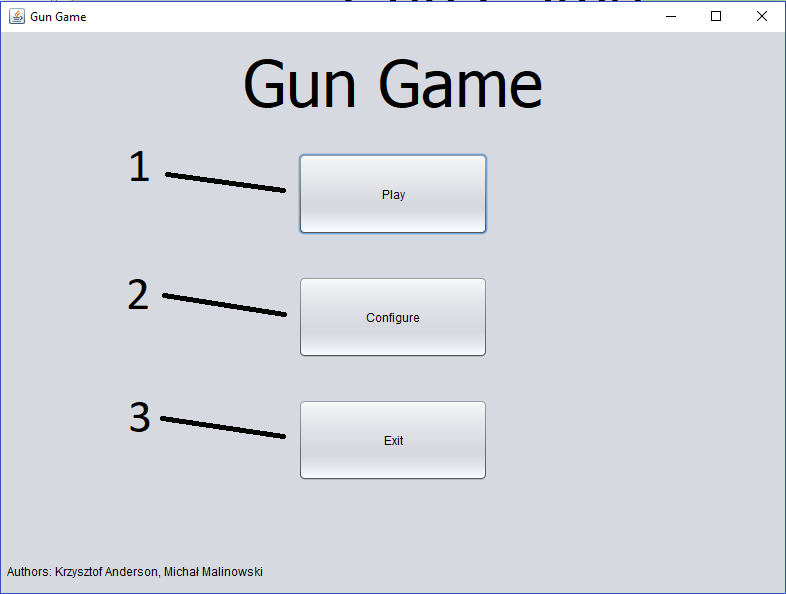
\includegraphics[width=14cm]{obrazy/mainmenuscreen.png}
    \caption{Główne menu}
    \label{main menu}
    \end{figure}
    \item Frame \code{GunGame} składa się z:
    \begin{itemize}
        \item pól tekstowych wyświetlających liczbę punktów każdego z graczy opisanych numerem 1;
        \item dwóch przycisków opisanych numerami 2 i 3, z własnymi słuchaczami akcji reagującymi na wciśnięcie, z czego przycisk 2 zatrzymuje grę i wywołuje dialog opisany w kolejnym punkcie, a przycisk 3 kończy działanie aplikacji;
        \item panelu gry, na którym znajdują się obiekty oznaczone numerami 4, 5 oraz 6, przy czym 4 to instancje klasy \code{Player}, 5 to instancje klasy \code{Missile} a 6 to instancje klasy \code{Block}.
    \end{itemize}
    Panel gry posiada słuchaczy akcji reagujących na wciśnięcie odpowiednich przycisków na klawiaturze, sterujących pojazdami gracza pierwszego i~drugiego. Wciśnięcie klawisza:
    \begin{itemize}
        \item A lub ; spowoduje wywołanie metody \code{moveLeft()},
        \item S lub ' spowoduje wywołanie metody \code{moveRight()},
        \item Z lub . spowoduje wywołanie metody \code{rotateLeft()},
        \item X lub / spowoduje wywołanie metody \code{rotateRight()},
        \item C lub , spowoduje wywołanie metody \code{fire()}.
    \end{itemize}
    \begin{figure}[H]
    \centering
    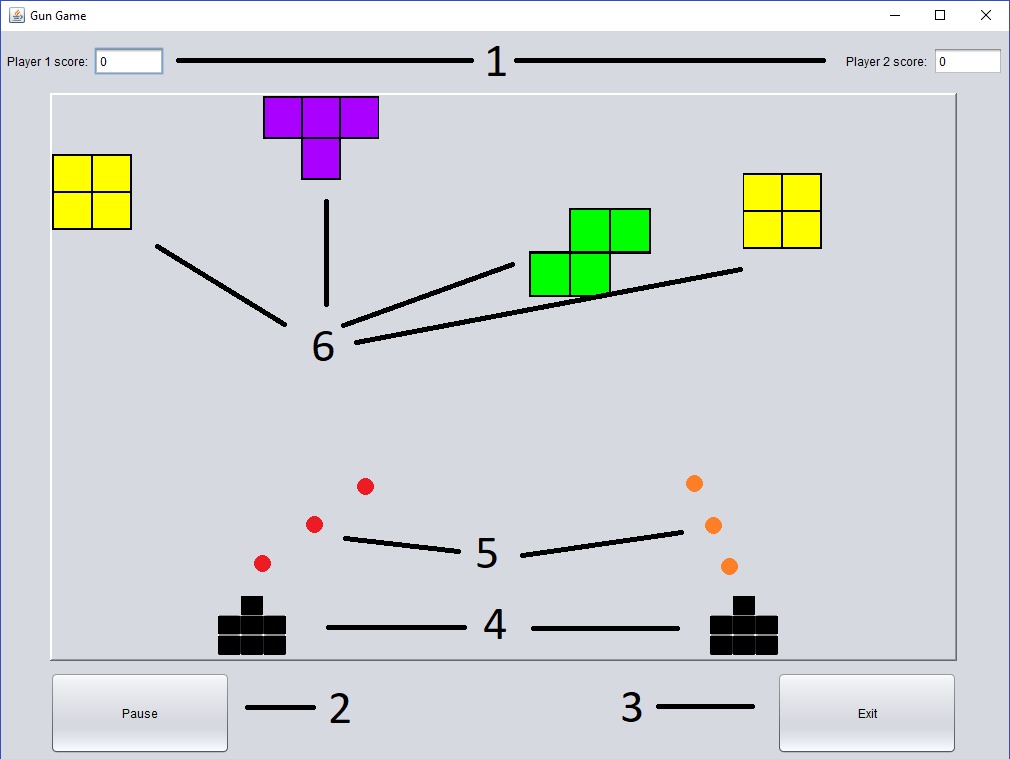
\includegraphics[width=14cm]{obrazy/gamescreen.png}
    \caption{Ekran gry}
    \label{Game screen}
    \end{figure}
    \item Dialog \code{Pause} składa się z 3 przycisków opisanych numerami 1, 2 oraz 3. Przycisk numer 1 zamyka dialog i wznawia rozgrywkę, przycisk numer 2 zapisuje obecną konfigurację do pliku tekstowego, a przycisk numer 3~wywołuje dialog \code{MainMenu}.
    \begin{figure}[H]
    \centering
    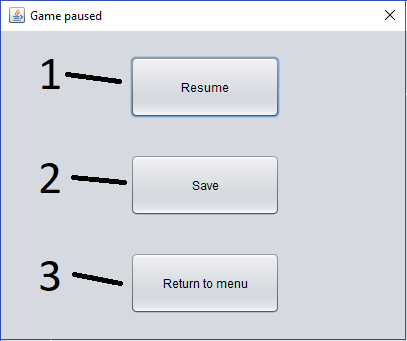
\includegraphics[width=14cm]{obrazy/pausemenuscreen.png}
    \caption{Ekran pauzy}
    \label{Pause menu}
    \end{figure}
\end{enumerate}
\section{Testowanie}
Program zostanie przetestowany na dwa różne sposoby.
\subsection{Testy jednostkowe}
Zostaną tu wykorzystane narzędzia udostępniane przez JUnit. Testy będą polegały na wprowadzeniu danych testowych do testowanych metod i sprawdzenie, czy wynik jest zgodny z oczekiwaną wartością.
\begin{itemize}
    \item \code{chceckCollisions} wprowadzone zostaną kolizyjne dane i sprawdzone zostanie czy metoda poprawnie na nie zareaguje.
    \item \code{getImageDimensions} zostanie wprowadzony do tej funkcji obraz o znanych rozmiarach i sprawdzone zostanie czy pola \code{width} i \code{height} zawierają poprawne wymiary obrazu.
    \item \code{getRandomNumber} wprowadzony zostanie zakres w którym ma zostać wylosowana liczba, następnie zostanie sprawdzone czy wylosowana liczba jest z danego zakresu. Test zostanie przeprowadzony 10 razy, aby kilkukrotnie wylosować nową liczbę i poddać ją badaniu.
    \item \code{readFile} wprowadzony zostanie plik o znanej zawartości i sprawdzone zostanie czy został on poprawnie odczytany.
    \item \code{writeFile} wprowadzony zostanie znany tekst i sprawdzone zostanie czy został on poprawnie zapisany do pliku.
\end{itemize}
\subsection{Testy akceptacyjne ręczne}
Będą one przeprowadzane przez twórców programu na działającym programie. Polegać będą na wymuszeniu nietypowych lub granicznych zachowań w~trakcie rozgrywki i sprawdzenie jak program się zachowa. Wynik niektórych testów będzie można określić przez obserwację zachowań obiektów graficznych w~programie.
\begin{itemize}
    \item Zostanie sprawdzone, czy można zmienić wymiary okienka w którym wyświetla się program, poprzez próby zmiany jego rozmiaru myszką.
    \item Zostanie sprawdzone, czy program odpowiednio reaguje na wprowadzenie niepoprawnego pliku konfiguracyjnego, poprzez wprowadzenie błędnego pliku konfiguracyjnego.
    \item Zostanie sprawdzone, czy poprawnie zostaną obsłużone wprowadzone błędne nazwy graczy, poprzez wprowadzenie błędnych nazw graczy.
    \item Zostanie sprawdzone, czy czołgi mogą poruszać się po planszy przy pomocy odpowiednich przycisków. Próbie zostanie poddane także poprawne reagowanie obrotu lufy na wciskane klawisze i strzelanie poprzez odpowiednią interakcję z programem.
    \item Zostanie sprawdzone, czy lufa nie jest w stanie obrócić się o kąt większy, niż podany w pliku konfiguracyjnym, poprzez próbę obrotu jej o kąt większy niż dozwolony.
    \item Zostanie sprawdzone, czy czołgi nie mogą przez siebie przenikać, ani wyjeżdzać poza planszę, poprzez próbę przeniknięcia przez siebie czołgów.
    \item Zostanie sprawdzone, czy dodawane są poprawne ilości punktów, poprzez zbijanie różnych klocków i obserwowanie zmian w wyniku gracza.
    \item Zostanie sprawdzone, czy przycisk pauzy poprawnie działa, poprzez zapamiętanie stanu rozgrywki, spauzowanie gry i ponowne jej uruchomienie. Kiedy rozgrywka będzie wyglądać tak samo, test zakończy się pozytywnie.
    \item Zostanie sprawdzone, czy zapisywanie gry działa poprawnie, poprzez zapisanie obecnego stanu rozgrywki, wyjście z programu i po ponownym uruchomieniu programu, wczytanie wygenerowanego pliku. Jeżeli stan rozgrywki będzie taki sam, test zakończy się pozytywnie.
\end{itemize}
\section{Diagram klas}
\begin{figure}[H]
    \centering
    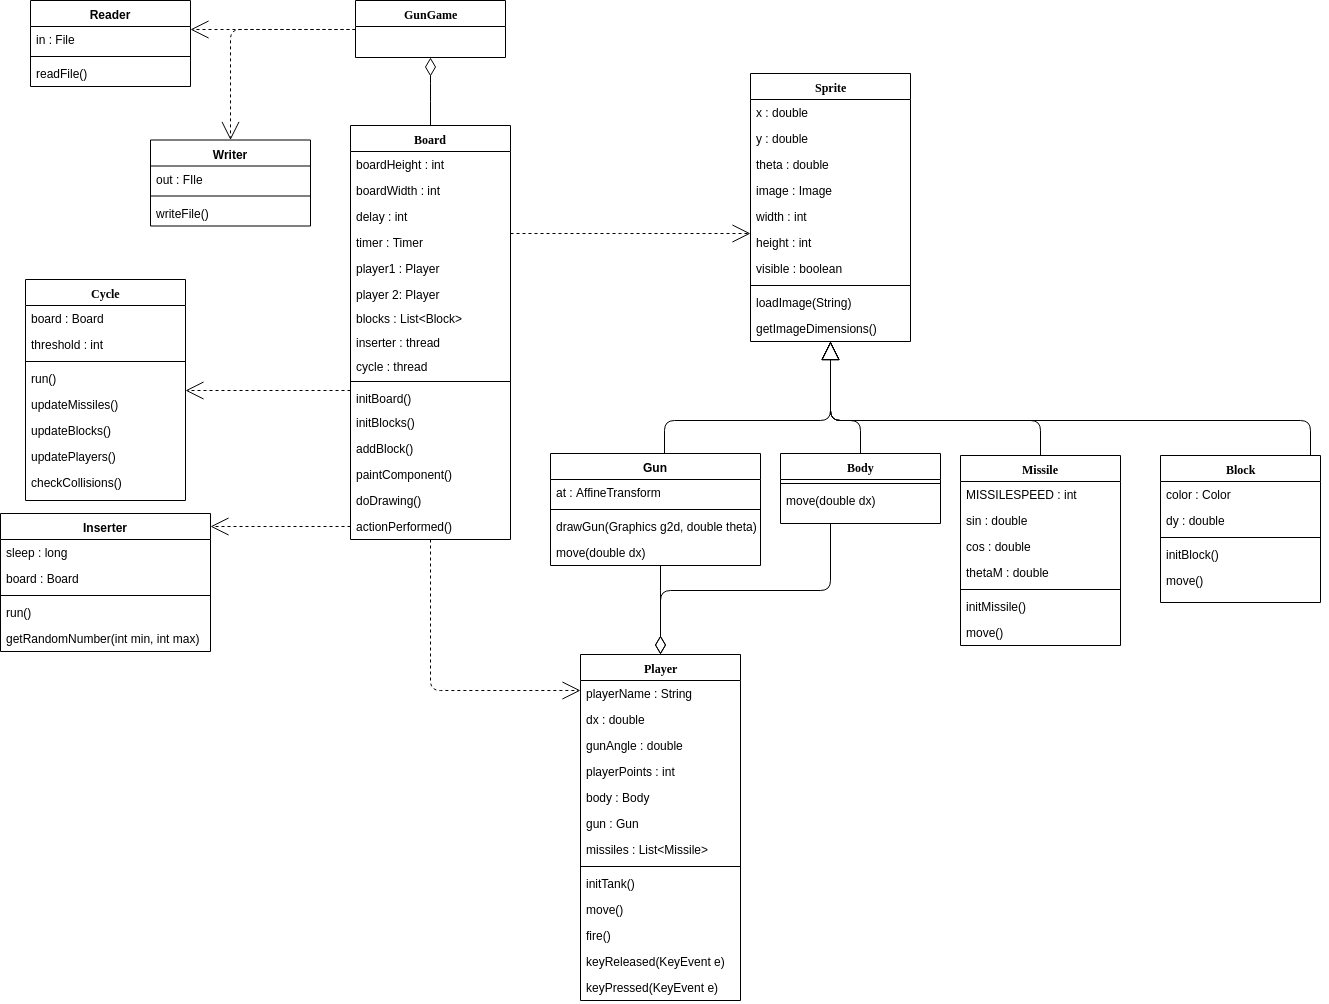
\includegraphics[width=20cm, angle=90]{obrazy/Diagram.png}
    \caption{Diagram klas}
    \label{diagram klas}
    \end{figure}
\end{document}




